\documentclass{report}

\usepackage[portuguese]{babel}

\usepackage[letterpaper,top=2cm,bottom=2cm,left=3cm,right=3cm,marginparwidth=1.75cm]{geometry}

% Useful packages
\usepackage{amsmath}
\usepackage{graphicx}
\graphicspath{ {./images/} }
\usepackage[colorlinks=true, allcolors=blue]{hyperref}
\usepackage{etoolbox}
\patchcmd{\abstract}{\null\vfil}{}{}{}

\usepackage{lipsum}


\title{Google TPU}
\author{Fernando Lima \\ Isabella Caselli \\ Rodrigo Michelassi}
\date{2024}

\begin{document}
\maketitle
\tableofcontents	% como colocar isso na mesma pagina que o titulo

% --- ABSTRACT --- % 
\begin{abstract}
Na era do desenvolvimento de sistemas baseados em Inteligência Artificial, se faz necessário o uso de máquinas super potentes, capazes de processar dados e realizar operações matemáticas de maneira extremamente rápida. Modelos de Machine Learning podem levar horas, até mesmo dias, para serem treinados, devido principalmente a operações como produto interno entre matrizes e a enorme quantidade de dados que são usados, trazendo um prejuízo não apenas de tempo, mas também energético, ambiental e sobretudo lucrativo. Nesse artigo, iremos tratar brevemente sobre a utilização de Cloud TPUs, unidades de processamento de tensores do Google Cloud, que atuam na otimização do treinamento de modelos de aprendizado de máquina, e que se tornou indispensável na academia e na indústria, para todos estudiosos e profissionais da área.
\end{abstract}

% --- CHAPTER 1 --- % 
\chapter{Introdução}

A evolução da tecnologia tem proporcionado diversos avanços no campo da inteligência artificial, principalmente no desenvolvimento de redes neurais profundas (Deep Learning) e aprendizado de máquina. Nesse cenário, a demanda por maior poder computacional levou à criação de hardware especializado, capaz de lidar com a complexidade e o volume de cálculos necessários para essas tarefas. Nesse contexto, destaca-se a Unidade de Processamento Tensorial (TPU), um circuito integrado de aplicação específica (ASIC) desenvolvido pelo Google.

As TPUs, lançadas em 2015, foram projetadas para acelerar operações de aprendizado de máquina, otimizando o treinamento de modelos baseados em redes neurais. Diferentemente de CPUs e GPUs, cuja arquitetura é projetada para fins generalistas, as TPUs são especializadas em multiplicações e somas de matrizes, que são operações fundamentais em áreas como Deep Learning. Essa especialização confere às TPUs maior eficiência energética e desempenho significativamente superior em tarefas relacionadas à inteligência artificial.

Dessa forma, considerando o tema apresentado como essencial para os avanços significativos que foram alcançados nas áreas de IA e Aprendizado de Máquina, este trabalho se propõe a explorar a arquitetura, os princípios de funcionamento e as aplicações das TPUs no contexto da computação moderna. 

% --- CHAPTER 2 --- % 
\chapter{História}

A Google Tensor Processing Unit é uma arquitetura de circuito integrado conhecido como um "acelerador de IA". Essa arquitetura tem seu início em $2016$, como uma alternativa a outras estruturas já conhecidas, utilizadas popularmente para acelerar o treinamento de modelos de IA, como as GPUs e os arrays sistólicos.

Apesar dessa tecnologia ser divulgada ao público apenas em $2016$, engenheiros da Google divulgaram que já era utilizada há mais de um ano em datacenters da big tech. Essa arquitetura foi pensada para funcionar juntamente a biblioteca de Machine Learning da Google, o TensorFlow, utilizada para treinar grandes modelos baseados em redes neurais, e atualmente uma das maiores bibliotecas do ramo. 

Entre as principais atividades executadas pela TPU está o processamento de tensores, estrutura de dados conhecida como um array multidimensional. Dessa forma, estratégias diversas para multiplicação de tensores (linear e paralelamente) são comumente estudadas em diversos campos da matemática clássica, dentro da Álgebra Linear, e as mais modernas arquiteturas para processamentos de produtos matriciais se baseiam em técnicas já conhecidas.

Atualmente, as TPUs são proprietárias, e no geral o acesso se limita a própria Google ou usuários que pagam por seu uso. É possível que empresas contratem o serviço por meio do sistema de nuvem da Google ou utilizem através do Google Colab, com tempo limitado de uso ou aluguel de TPUs mais potentes.

% --- CHAPTER 3 --- % 
\section{Tensores}

% --- CHAPTER 4 --- % 
\section{Modelos de Aprendizado de Máquina}

Nos tempos de ChatGPT, IA's generativas, problemas éticos com uso de imagens e dados pessoais por grandes empresas, surge a necessidade de se entender como funcionam os modelos de Aprendizado de Máquina. 

Nesse sentido, o surgimento das TPUs estão associadas justamente oa fortalecimento científico e comercial desse tipo de tecnologia, que a cada dia vem sendo explorada mais fortemente, e utilizando grandes camadas de dados. Esses modelos exigem muito poder computacional para processar todos os dados fornecidos, além de realizar diversas operações matemáticas como produtos tensoriais. 

De maneira resumida, modelos de Aprendizado de Máquina no geral consiste na modelagem matemática de problemas, com propósitos variáveis, mas que todos possuem algo em comum: fazer com que o modelo se ajuste bem, a ponto de dar respostas boas para suas entradas. Dessa forma, se percebe uma boa semelhança com a computação clássica, dada uma entrada, processamos uma respectiva saída. Todavia, esses modelos são probabilísticos, e não há garantia que a resposta sempre será a esperada. Para que servem esses modelos, então?

Há problemas que são fáceis para humanos responderem, mas difíceis de serem automatizados. Por exemplo, dada uma imagem de um gato, um ser humano pode facilmente ver a imagem e dizer "essa é uma imagem de um gato". Porém, se existisse a necessidade de automatizar tal tarefa? Como podemos escrever um algoritmo que, dada uma imagem, de qualquer tamanho e padrão de cores, apenas utilizando ferramentas clássicas de algoritmos (loops, condicionais) e dizer se aquela imagem contém de fato, um gato? Nesse contexto, utilizar Machine Learning é uma boa ideia.

Adicionalmente, os modelos mais modernos de Aprendizado de Máquina estão atrelados ao desenvolvimento de redes neurais. Esses modelos são treinados baseados em dois passos, conhecidos como forward e back-propagation. Redes Neurais são constituídas por nós, representando features de dados, e pesos atribuídos a cada uma dessas features, e a operação de Forward-Propagation consiste em realizar produtos vetoriais entre esses pesos com o valor dos nós. A operação de Back-Propagation deve retornar a rede neural, atualizando os pesos com base no erro calculado, novamente utilizando operações de produtos vetoriais. Note que essas operações são extremamente custosas, e Redes Neurais possuem milhares, até milhões de parâmetros, a depender do modelo, e é necessário acelerar esse processamento, com base em paralelismo e busca de algoritmos mais eficientes.

\begin{figure}[h]
	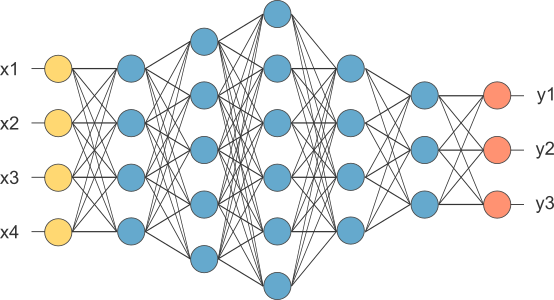
\includegraphics[scale=0.5]{neuralNetwork}
	\centering
	\caption{Estrutura gráfica de uma Rede Neural}
\end{figure}

Com base nisso, temos um modelo matemático, que atualiza pesos e é capaz de responder perguntas, porém se ele nem sempre acerta, como eles são de fato utilizados? Vimos que modelos de Aprendizado de Máquina são baseados matemáticos e baseados em pesos. Existem diversas aplicações para esses modelos, e o trabalho de um engenheiro de Machine Learning é conseguir treinar um modelo, com dados o suficiente, de forma a minimizar o erro desse modelo, dessa forma aumentando sua acurácia e garantindo que o modelo tenha uma maior probabilidade de acertar as respostas, com base nos dados que são utilizados como entrada. Atualmente, esses modelos tem diversos usos na indústria, como no mercado financeiro, para predição de séries temporais para variações da bolsa de valores, na medicina para auxílio de profissionais no diagnóstico de doenças, no direito para análise textual de casos, na astronomia, como na recente descoberta da primeira imagem de um buraco negro. 

Dessa forma, Machine Learning é uma tendência que cresce tanto no mercado como na academia, e deve continuar sendo explorado por diversos profissionais, de forma que é necessário acelerar o longo processo de treinamento de modelos, além de buscar soluções mais sustentáveis para que o conhecimento possa continuar se expandindo.


% --- CHAPTER 5 --- % 
\chapter{Arquitetura da TPU}

% --- CHAPTER 6 --- % 
\chapter{TPU vs GPU}

% --- CHAPTER 7 --- % 
\chapter{TensorFlow}

% --- CHAPTER 8 --- % 
\chapter{Cloud TPU v5p}

Como discutido anteriormente, LLMs são os novos modelos mais explorados no mercado e na academia. Todavia, esses modelos utilizam dados de toda (ou quase toda) a internet, que cresce ainda mais exponencialmente. Todos os dias há milhões de novos dados sendo gerados. Dessa forma, é importante que o hardware acompanhe o crescimento na quantidade de dados disponíveis, de forma que seja possível possuir poder computacional suficiente para treinar modelos como esses.

Com isso em vista, a evolução das TPUs deve ser rápida, portanto, em 2023, a Google apresentou, em 2023, a v5p, a TPU mais poderosa da empresa. Com esse lançamento, a Google prometeu a entrega de uma performance até $2.8$ vezes mais rápida, utilizada para alimentar ecossistemas internos da multinacional, como o Youtube, Android e Gmail.

Essa TPU se diferencia das demais, pois é focada em desempenho possível, sem levar em consideração a facilidade operacional. Um grande diferencial é a forma como a TPU lida com operações em ponto flutuante. Por dados oficiais da Google, essa arquitetura traz $8960$ chips e três vezes mais memória HBM.

\begin{figure}[h]
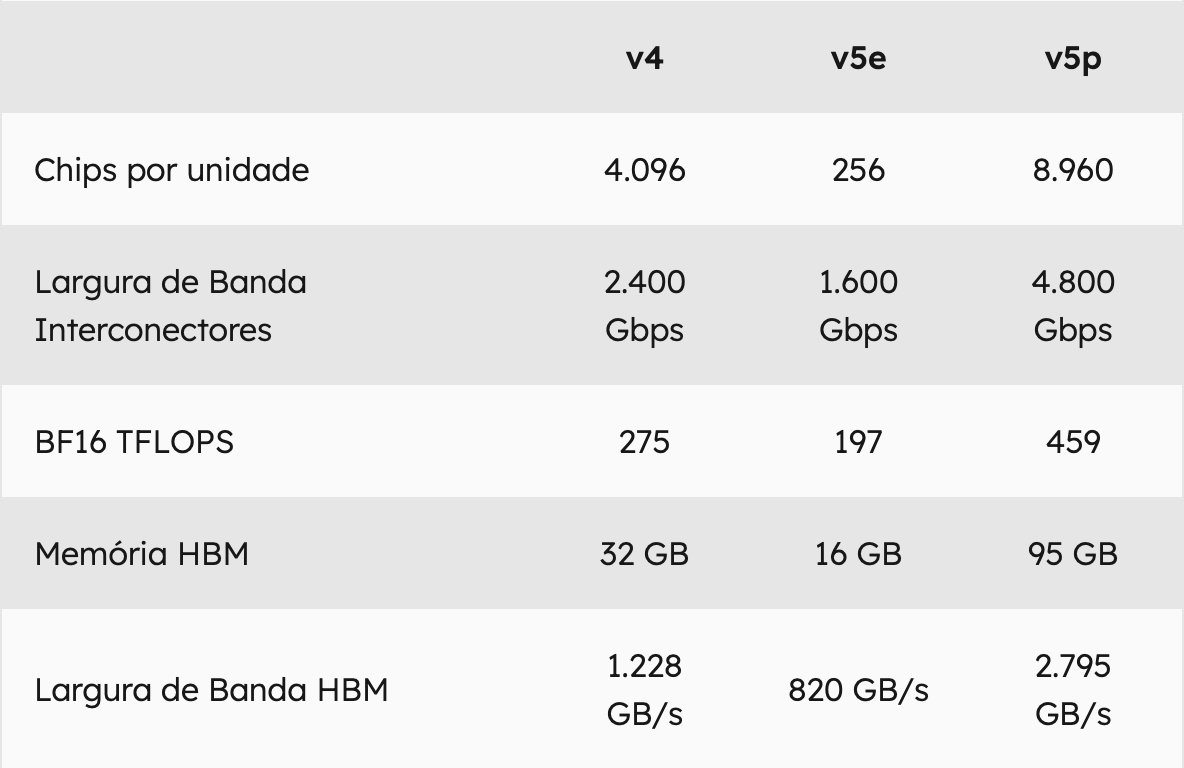
\includegraphics[scale=0.5]{comparativo-tpus}
\centering
\caption{Comparativo entre TPUs Google para cargas de trabalho em IA e LLM}
\end{figure}

Mas no fim, o que significam esses valores? A Google promete que a nova TPU consegue escalar o tempo de treinamento, sendo até $4X$ mais rápida que TPUs mais baratas, como a $V4$, devido ao dobramento no tamanho de operações em ponto flutuante que são entregues.

% --- CHAPTER 9 --- % 
\chapter{Google Colab e distribuição}

\bibliographystyle{alpha}
\bibliography{sample}

\href{https://www.run.ai/guides/cloud-deep-learning/google-tpu}{TPU e Arquitetura}

\href{https://cloud.google.com/blog/products/compute/performance-per-dollar-of-gpus-and-tpus-for-ai-inference}{Comparativos oficiais em modelos de IA (TPU vs GPU)}

\href{https://canaltech.com.br/inteligencia-artificial/cloud-tpu-v5p-e-o-novo-e-mais-poderoso-acelerador-de-ia-do-google-272299/}{TPU v5p}

\href{https://cloud.google.com/tpu?hl=pt-BR}{Conceitos básicos}

\href{https://en.wikipedia.org/wiki/Tensor_Processing_Unit}{Wikipedia, tem tudo}

\href{https://arxiv.org/pdf/1704.04760}{Paper original da TPU}

\end{document}